\subsection{Mean Squared Error (MSE)}

\indent 

The MSE measures the average squared difference between the predicted values and the true values:

\begin{align*}
    \text{MSE} = \mathbb{E}[(Y-\hat{f}(X))^2]
\end{align*}

\textbf{MSE Can Be Decomposed Into Three Components:}

\begin{align*}
    \text{MSE} = \mathbb{E}[(y_0-\hat{f}(x_0))^2] = \text{Bias}^2+\text{Var}(\hat{f}(x_0))+\text{Var}(\epsilon)
\end{align*}

\subsubsection{Bias-Variance Tradeoff}

\indent

\noindent \textbf{High complexity/flexibility model}: 

\begin{itemize}
    \item \textbf{Low bias}: fits the training data well, overfits.
    \item \textbf{High variance}: sensitive to noise.
\end{itemize}

\noindent\textbf{Low complexity/flexibility model}:

\begin{itemize}
    \item \textbf{High bias}: too simple, underfits.
    \item \textbf{Low Variance}: more stable across different samples.
\end{itemize}

\subsection{Classification}

\subsubsection{Basic Principles}

\indent 

Each observation consists of class label $y$ (categotical variable) and feature vector $\boldsymbol{x} = (x_1,x_2,...,x_p)$ (mix of categorical and continuous variables).

Goal is to classify $y$ using $\boldsymbol{x}$. Classification models produce a continuous valued prediction, which is usually in the form of a probability (i.e., the predicted values of class membership for any individual sample are between 0 and 1 and sum to 1). It require a rule to assign observations to a category based on the predicted probability.

\subsubsection{Classification vs Clustering}

\indent 

\noindent\textbf{Classification}: classes are predefined, want to use a training set of labeled objects to form a classifier for classification of future observations (supervised)

\noindent\textbf{Clustering}: classes are unknown, want to discover them from the data (unsupervised)

\subsubsection{Two class classification (Binary)}

\indent 

Binary in there are two possible values (0 or 1, TRUE or FALSE).

\noindent\textbf{Linear regression misspecifications}: The regression line $\beta_0+\beta_1x$ can span the entire real line, all values between $-\infty$ to $+\infty$. For the target variable $y$ only takes two values: 0 or 1, the linear regression model is not well specified for this purpose.

\subsection{Logistic regression}

\indent 

The multiple regression could write as $\mathbb{E}[Y|X] = \boldsymbol{X\beta}$.

\begin{align*}
    Y & = \boldsymbol{X\beta}+\epsilon\\
     & = \beta_0 + \beta_1X_1+...+\beta_pX_p+\epsilon
\end{align*}

This can generalise this to $g(\mathbb{E}[Y|X]) = \boldsymbol{X\beta}$.

Logistic regression is a special case of one of these generalised linear models:

\begin{align*}
    \log(\frac{p}{1-p}) = \boldsymbol{X\beta}, p = P(Y=1|X)
\end{align*}

Dolve for $p$ gives:

\begin{align*}
    p = g^{-1}(\boldsymbol{X\beta}) = \frac{1}{1+\exp{(-\boldsymbol{X\beta})}}
\end{align*}

\subsubsection{Terminology}

Logistic function responsible from mapping the features from $(-\infty,+\infty) = \mathbb{R}$ to $(0,1)$.

we want the values in the logit space to be linear in $\boldsymbol{X}$, We choose 
$\beta$ that minimizes the negative log-likelihood (log-loss):

\begin{align*}
    \ell(\beta) = \sum_{i=1}^n -y_i\log(p(x_i)) - (1-y_i)\log(1-p(x_i))
\end{align*}

Gradient-descent methods can be used for optimization.

Decision boundary: predict $Y=1$ if $\boldsymbol{X\beta}\geq 0$.

\subsection{Linear Discriminant Analysis (LDA)}

\indent 

LDA classifies data by finding the decision boundary that best separates different classes, assuming the data follows Gaussian distributions with a class specific mean $(\mu_k)$ and a common variance $(\sigma^2)$.

\subsubsection{Bayes’ Theorem in the classification context}

\begin{align*}
    p_k(x) = P(Y=k|X=x) = \frac{\pi_kf_k(x)}{\sum_{i=1}^K\pi_\ell f_\ell (x)}
\end{align*}

$f_k(x)$ is the density function for feature $x$ given it’s in group $k$.

\begin{itemize}
    \item Posterior: The probability of classifying observation to group $k$ given it has features $x$.
    \item Prior: The prior probability of an observation in general belonging to group $k$
\end{itemize}

\subsubsection{LDA setup}

\indent 

Using the Bayes’ Theorem, we model:

\begin{align*}
    & p_k(x) = P(Y=k|X=x) = \frac{\pi_kf_k(x)}{\sum_{i=1}^K\pi_\ell f_\ell (x)}\\
    & \pi_k: \text{Probability of coming from class $k$ (prior probability)}\\
    & f_k(x): \text{Density function for $X$ given that $X$ is an observation from class $k$}
\end{align*}

This is a generative approach that models the distribution of each class (assuming Gaussian distributions) and then uses Bayes’ theorem to find the decision boundary.

\subsubsection{Estimation of $\pi_k$ and $f_k(x)$}

\indent 

We can estimate $\pi_k$ and $f_k(x)$ to compute $p_k(x)$. The most common model for $f_k(x)$ is the Normal Density $N(\mu_k,\sigma_k^2)$.

If we use the above density, we only need to estimate $3$ quantities to compute $p_k(x)$: $\mu_k, \sigma_k^2, \pi_k$.

For simplicity, we assume common variance $\sigma = \sigma_1 = ...=\sigma_k = ...$.

We can allow the observations in the $k$-th class to have a class-specific variance $\sigma_k^2$, leading to the quadratic discriminant analysis.

\begin{itemize}
    \item The mean $\mu_k$ could be estimated by the average of all training observations from the $k$-th class.
    \item The variance $\sigma^2$ could be estimated as the weighted average of variances of all $K$ classes.
    \item The poportion $\pi_k$ could be estimated as the proportion of the training observations that belong to the $k$-th class.
\end{itemize}

Here, $n $ is the sample size, $n_k$ is the number of samples in the $k$-th class.

\begin{align*}
    & \hat{\mu}_k = \frac{1}{n_k}\sum_{i:y_i = k}x_i\\
    & \hat{\sigma}^2 = \frac{1}{n-K}\sum_{k=1}^K\sum_{i:y_i = k}(x_i - \hat{\mu}_k)^2\\
    & \hat{\pi}_k = \frac{n_k}{n}
\end{align*}

\subsubsection{Why LDA?}

\indent 

In the case where \textbf{$n$ is small, and the distribution of predictors $X$ is approximately normal}, then LDA is more stable than Logistic Regression. 

LDA is more popular when we have \textbf{more than two response classes}. More intuitive to predict class assignment. But logistic regression CAN be generalised for classification problems with more than two classes.

When classes are \textbf{perfectly separated}, the parameter estimates in logistic regression become infinite. This can lead to instability in software (e.g., R) when estimating parameters. In contrast, LDA remains stable and does not face this issue.

LDA may perform poorly for categorical predictors due to the normality assumption.

\subsubsection{Logistic Regression vs LDA}

\indent 

\noindent\textbf{Similarity:}

Both Logistic Regression and LDA produce \textbf{linear boundaries}.

\bigskip

\noindent\textbf{Differences:}

\begin{itemize}
    \item LDA assumes that the observations are drawn from the normal distribution with common variance in each class, while logistic regression does not have this assumption.
    \item LDA would do better than Logistic Regression if the assumption of normality hold, otherwise logistic regression may outperform LDA
\end{itemize}

\subsection{$k$-Nearest Neighbours (kNN)}

\indent 

The kNN model computes the probability of an observation with features $x$ belonging to group $\ell$ based on the membership of the nearest points (denoted by $N_x^k)$ to $x$.

\begin{align*}
    P(Y = \ell|x) = \frac{1}{k}\sum_{i\in N_x^k}1_{\{y_i = \ell\}}
\end{align*}

Here $\sum_{i\in N_x^k}1_{\{y_i = \ell\}}$ counts of the closest $k$ points that belong to group $\ell$.

\subsubsection{kNN vs LDA and Logistic Regression}

\indent 

kNN is \textbf{completely non-parametric}: No assumptions are made about the shape of the decision boundary.

\noindent \textbf{Advantage}:

We can expect kNN to dominate both LDA and Logistic Regression when the decision boundary is highly non-linear.

\bigskip

\noindent\textbf{Disadvantage}:

\begin{itemize}
    \item kNN does not tell us which predictors are important (no table of coefficients).
    \item The choice of the number of $K$ matters.
\end{itemize}

\subsection{Support Vector Machines (SVM)}

\indent 

SVM finds a decision boundary (hyperplane) that best separates the two classes by maximising the margin between them.

\textbf{Support vectors}: observations that either lie on or violate the margin

\subsubsection{Hyperplane}

\indent 

In $p$ dimensions, it is a flat affine subspace of dimension $p-1$.

For the general equation: $\beta_0 + \beta_1X_1+...+\beta_pX_p = 0$. If $\beta_0=0$, the hyperplane passes through the origin, otherwise it does not. The vector $(\beta_1,\beta_2,...,\beta_p)$ is called the normal vector - It points in a direction orthogonal to the surface of the hyperplane.

\subsubsection{Separating hyperplanes}

\begin{figure}[h]
    \centering
    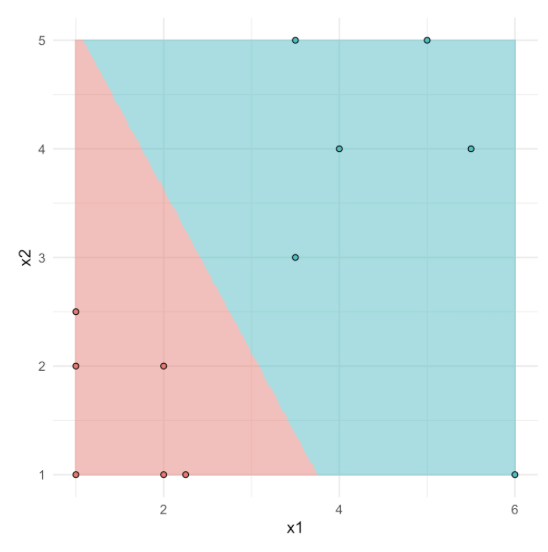
\includegraphics[width=0.5\linewidth]{Figure/Week 5/Separating hyperplanes.png}
\end{figure}

Consider coding Red as $y_i=-1$ and blue as $y_i=1$, then $y_if(x_i)>0$ for all $i$, $f(x_i)$ defines a separating hyperplane.

If $f(x_i) = \beta_0 + \beta_1X_1+...+\beta_pX_p$ defines a hyperplane, $f(x)>0$ defines a region on one side of the hyperplane, $f(x)<0$ defines another.

\subsubsection{Margin}

\indent 

\noindent\textbf{Maximal Margin Classifier}:

\begin{align*}
    \max_{\beta_0,...,\beta_p} M \text{ such that} &\sum_{j=1}^p\beta_j^2 = 1\\
    & y_i(\beta_0+\beta_1x_{i1}+...+\beta_px_{ip})\geq M, i = 1,...,n
\end{align*}

\bigskip

\noindent\textbf{Soft margin}:

\begin{figure}[h]
    \centering
    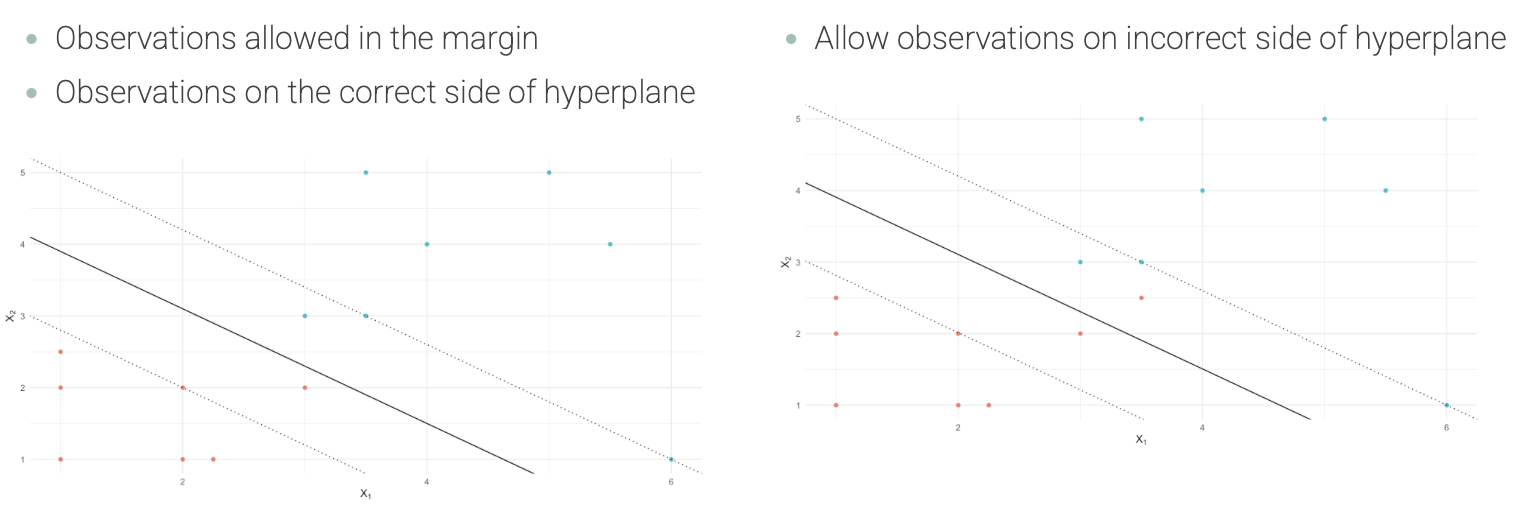
\includegraphics[width=0.8\linewidth]{Figure/Week 5/Soft margin.png}
\end{figure}

If a basic mathematical plane is not possible due to non-perfect separation or outliers, we introduce a soft margin to relax the requirement for all observations to be on the correct side of the margin.

\subsubsection{Support Vector Classifier}

\indent 

Support Vector Classifier solves the following optimization problem:

\begin{align*}
    \max_{\beta_0,...,\beta_p,\epsilon_1,...,\epsilon_n}M \text{ such that } & \sum_{j=1}^p \beta_j^2 = 1\\
    & y_i(\beta_0+\beta_1x_{i1}+...+\beta_px_{ip})\geq M(1-\epsilon_i), i =1,...,n\\
    & \epsilon_i \geq0, i = 1,...,n, \sum_{i=1}^n\epsilon_i\leq C
\end{align*}

Here:

\begin{itemize}
    \item $C$ is a non-negative tuning parameter.
    \item $M$ is the width of the margin.
    \item $\epsilon_i$ are slack variables that allow observations to be on the wrong side of the margin.
    \begin{itemize}
        \item if $\epsilon_i>1$, then observation $i$ is on the wrong side of the hyperplane
        \item if $0<\epsilon_i\leq 1$, then observation $i$ is on the correct side but inside margin
        \item if $\epsilon_i = 0$, then observation $i$ is on the correct side and past the margin
    \end{itemize}
\end{itemize}

\subsubsection{Feature space expansion}

\indent 

Enlarge the space of features by including transformations:

\begin{itemize}
    \item new features that are powers and products $X_1^2,X_1^3,X_1X_2$
    \item Hence go from $p$-dimensional space to $P>p$ dimensional
\end{itemize}

Fit (linear) support vector classifier in the expanded feature space. Impact is a non-linear decision boundary in original feature space. This leads to non-linear decision boundary in the original space (quadratic conic sections).

For example, Suppose we start off in 2-dimensional feature space $(X_1,X_2)$. We make new feature space $(X_1,X_2,X_1^2,X_2^2,X_1X_2)$. Then the decision boundary would be of the form: $\beta_0+\beta_1X_1+\beta_2X_2+\beta_3X_1^2+\beta_4X_2^2+\beta_5X_1X_2 = 0$.

\subsubsection{Non-linearity and kernels}

\indent 

Polynomials add complexity and scale poorly in high dimensions. Kernels allow us to introduce non-linearity efficiently without explicitly adding features. The inner product trick enables the SVCs to classify non-linear data in an elegant and computationally efficient way.

\subsubsection{Inner products and support vectors}

\indent 

Recall $\boldsymbol{x}_i = (x_{i1},x_{i2},...,x_{ip})\in\mathbb{R}^p$.

Inner product between vectors given by:

\begin{align*}
    \langle \boldsymbol{x_i},\boldsymbol{x_j}\rangle = \sum_{k=1}^px_{ik}x_{jk}
\end{align*}

Recall the hyperplane equation $f(x) = \beta_0+\beta_1x_1+...+\beta_px_p$.

The linear support vector classifier can be represented as:

\begin{align*}
    f(x) = \beta_0+\sum_{i=1}^n \alpha_i\langle \boldsymbol{x},\boldsymbol{x_i}\rangle
\end{align*}

\subsubsection{Support set}

\indent 

The parameters $\alpha_1,\alpha_2,...,\alpha_n$ and $\beta_0$ are estimated based on the inner products between pairs of training observations.

$\hat{\alpha}_i$is non-zero only for the support points $x_i$ (i.e., ones that lie on the margin), otherwise it equals to zero.

\begin{align*}
    f(x) = \beta_0+\sum_{j\in S}\alpha_j\langle\boldsymbol{x},\boldsymbol{x_i}\rangle
\end{align*}

Here, $S$ is the support set of indices such that $\alpha_i>0$

\subsubsection{Kernel functions}

\indent 

Suppose now we replace the inner product with a generalized function of the form $K(\boldsymbol{x}_i,\boldsymbol{x}_j)$. This function is called a kernel.

In this context, the kernel quantifies the similarity of two observations:

\begin{align*}
    &\text{Polynomial kernel} & K(\boldsymbol{x}_i,\boldsymbol{x}_j) = (1+\langle\boldsymbol{x}_i,\boldsymbol{x}_j\rangle)^d\\
    &\text{Gaussian radial kernel} & K(\boldsymbol{x}_i,\boldsymbol{x}_j) = \exp(-\gamma\sum_{k=1}^p(x_{ik}-x_{jk})^2)
\end{align*}

\subsubsection{SVM with more than two classes}

\indent 

SVM covered previously are design for binary classification. To expand this to $K$ classes there are two options.

\bigskip

\noindent\textbf{One vs all}:

Fit $K$ different binary classfiers, $f_k(x)$ for $k=1,2,...,K$ where each boundary attempts to separate class $k$ vs the rest.

Then $x_i$ is classified to $k^*$ where $f_{k^x}(x_i)>f_j(x_i)$ for all $j\neq k^*$ (i.e., the largest distance from the boundary).

\bigskip

\noindent\textbf{One vs one}:

Fit all $\binom{K}{2}$ pairwise classifiers. 

Fit $x_i$ to the class that wins the most pairwise comparisons.

\bigskip

\noindent Which to use?

If $K$ is small, do one vs one. Otherwise recommended one vs all.